\chapter{Forforstærker}

Forforstærkeren har til opgave at forstærke mikrofonens udgangssignal til et linjesignals niveau. Et linjesignal har en amplitude fra 200 mV til 2 V og mikrofonens udgangssignal ligger, ifølge standarderne, mellem 0.8 mV og 200 mV. Mikrofonens og linjesignalets spændingensområde er ikke proportionale, hvilket gør at mikrofonens udgangsspænding ikke kan forstærkes med en konstant faktor for at nå linjeniveau. Derfor er der valgt at tage udgangspunkt i én bestemt mikrofon i forforstærkerens design.
Mikrofonen, som vil blive brugt, er en Monacor MCE-4000 \fixme{ref til MCE4000 datablad}. Eftersom den valgte mikrofon er til at montere på PCB, og altså ikke en færdig mikrofon, skal der også designes styrekredsløb til denne. Kravene som valget af mikrofon tilføjer til forforstærkerens design samt kravene fra kravspecifikationen er vist i tabel \ref{tab:krav_forforstaerker}. 

\begin{table}[h]
\centering
\begin{tabular}{l|r|l}
\hline\hline
Område & Krav & Baggrund for krav \\
\hline\hline
Total Harmonic Distortion & \color{red}{<1 \%} & Ref til THD afsnit \\
Udgangssignaltype & Mono & Se afsnit \ref{krav_udgangssignaltype} \\
Forstærkning & Fra mikrofonens udgangsspænding til linjeniveau ( 200 mV - 2 V) & \\
\textbf{Frontpanel:} & & \\
Indgangsvælger & Ja & Se afsnit \ref{krav_indgangsvaelger} \\
\textbf{Fjernbetjening:} & & \\
Indgangsvælger & Ja &  Se afsnit \ref{krav_fjernbetjening}\\
\hline\hline
\end{tabular}
\caption{Krav fra kravspecifikationen som har indflydelse på forforstærkeren}
\label{tab:krav_forforstaerker}
\end{table}



\section{Design}


Mikrofon kan maksimalt levere en outputspænding på 18 mV. Forforstærkeren skal forstærke dette til linjeniveau hvormed forstærkningen bliver: $2/18*10^(-3)=111$. Derfor er der valgt at benytte to CE med uafkoblet Re trin: ét der forstærker 10 gange og ét der forstærker 11,1 gange. Dette er vist på figur \ref{blok_forforstaerker}.

\begin{figure}[h]
\centering
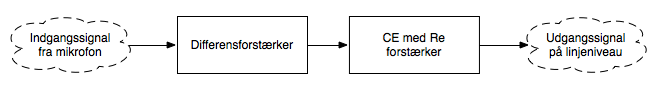
\includegraphics[scale=.6]{implementering/forforstaerker/blok_forforstaerker.png}
\caption{Blokdiagram over forforstærkerens byggeblokke samt lydsignalets vej}
\label{blok_forforstaerker}
\end{figure}

Udregningerne kan ses i vedlagt pdf (beregning-forforstaerker.pdf). 


\section{Simulering}


\section{Accepttest}

